\chapter{Ablauf der Fallstudie}\label{sec:fallstudie}

Da die Testautomatisierung bei einem verteilten, adaptiven System sehr aufwändig werden kann, soll nun ein modellbasierter Ansatz genutzt werden. Als reales System wurde Apache\texttrademark Hadoop\textregistered\footnote{\url{https://hadoop.apache.org/}} ausgewählt, welches mit einer adaptiven Komponente erweitert wurde. Von Hadoop sollen nun einige relevante Komponenten als Modell nachgebildet werden und anschließend mit einem realen Hadoop-Cluster verbunden werden. Dadurch soll der Ansatz des modellbasierten Testen auf ein reales System übertragen werden. Ebenfalls eine Rolle spielen einige Hauptprobleme wie \zB die Einbindung des realen Systems in das Modell oder der Umgang mit asynchronen Prozessen bei verteilten Systemen.

\section{Ablauf der Fallstudie}\label{sec:ablauf}

%Nun gibt es zahlreiche \ac{MC}, wie \zB \emph{LTSmin}\footnote{\url{http://fmt.cs.utwente.nl/tools/ltsmin/}}. Auch am \isse der Universität Augsburg wurde in den letzten Jahren mit \sS\footnote{\url{https://safetysharp.isse.de}} (sprich \emph{Safety Sharp}) ein entsprechendes Framework zum testen von sicherheitskritischen und selbst-adaptiven Systemen basierend auf dem \ac{MC}-Ansatz entwickelt \cite{Habermaier2015,Habermaier2016}. Nun ist das aktuelle Vorhaben, mithilfe von \sS ein reales Serversystem zu testen, welches bereits als theoretisches Modell basierend auf der ZNN.vom-Fallstudie, bekannt aus der Dissertation von Shang-Wen Cheng \cite{Cheng2008}, implementiert wurde. Als reales System soll nun \emph{Apache Hadoop}\footnote{\url{https://hadoop.apache.org/}} getestet werden, welches in der Industrie im Bereich Datenverarbeitung eingesetzt wird. Mit Hadoop ist es möglich, ein Servercluster zu erstellen, auf dem anschließend dafür entwickelte Anwendungen ausgeführt werden und somit große Datenmengen zu verarbeiten. Es soll daher nun getestet und analysiert werden, wie sich Hadoop unter verschiedenen Lastprofilen verhält und dabei bestimmte Fehler auftreten, wenn \zB einer der Hadoop-Nodes ausfällt.

%Bei der ZNN.com-Fallstudie als reines Modell gab es bereits eine ähnliche Aufgabenstellung, welche im Positionspapier \cite{Eberhardinger2017} genauer erläutert wurde. Das Hauptziel dieses Projektes ist daher nun, anstatt eines reinen Modells ein reales System zu testen. Dafür wird ein modellbasierter Ansatz als Testkonzept genutzt und Hadoop zunächst als Modell nachgebildet. Dieses Modell wird dann dazu genutzt, um ein reales Hadoop-Cluster entsprechend zu steuern und mithilfe des \ac{MC}-Ansatzes zu testen, wie sich das reale System unter bestimmten Bedingungen verhält und dabei zu ermitteln, wann es nicht mehr funktionsfähig ist.

\subsection{Aufbau des Modells}\label{sec:modellaufbau}

Zunächst muss natürlich erst einmal der Versuchsaufbau selbst in \sS modelliert werden. Ein Modell beinhaltet in \sS zunächst einmal die Komponenten des Systems und deren Zusammenhänge, also wie die Komponenten miteinander agieren. Wichtig sind in einem \sS-Modell aber auch mögliche Komponentenfehler, welche bekannt sind und jederzeit auftreten können. Komponentenfehler werden bereits in der Designphase eines Modells eingearbeitet und können bei der späteren Ausführung flexibel aktiviert und deaktiviert werden, um die Probleme des zu testenden Systems zu ermitteln (vgl. \autoref{sec:sSharp}).

Um nun Hadoop in \sS zu modellieren wird zunächst ein Konzept erstellt, in dem ausgearbeitet wird, welche Komponenten und Komponentenfehler relevant sind. Anschließend müssen deren Zusammenhänge und wesentlichen Eigenschaften ausgearbeitet werden und in das Konzept übernommen werden. Sobald das Konzept fertig ausgearbeitet ist, kann das Modell in \sS implementiert werden.

\subsection{Mapping zum realen System}\label{sec:mapping}

Nachdem die Basis des Modells steht, kann die Funktionalität entwickelt werden. Dazu werden in \sS nur Basisfunktionen eingebaut, um mit dem realen System kommunizieren zu können. Um für das reale System möglichst viele Ressourcen zur Verfügung zu stellen, wird das reale System auf einem eigenen PC installiert. Die Verbindung zwischen Modell und realem System wird mit einer Art Treiber realisiert, welcher mithilfe von mehreren SSH-Verbindungen mit dem realen Hadoop-Cluster kommuniziert und so das Mapping zwischen Modell und realem System übernimmt. Jede der SSH-Verbindungen ist dabei nur für einen Einsatzzweck gedacht, sodass es Verbindungen für \uA folgende Einsatzzwecke gibt:

\begin{itemize}[noitemsep]
	\item Starten von Benchmark-Anwendungen
	\item Monitoring des realen Cluster
	\item Injektion von Komponentenfehler
\end{itemize}

Der Vorteil von mehreren Verbindungen liegt darin, dass jede Verbindung unabhängig ist und nicht auf die Antwort des zuvor ausgeführten Befehls einer anderen Verbindung warten muss. So ist es möglich, mithilfe mehrerer Verbindungen mehrere Anwendungen parallel zu starten und jede Rückgabe auszuwerten und währenddessen verschiedene Komponentenfehler zu aktivieren.

\subsection{Erstellung der Lastprofile}\label{sec:lastprofilerstellung}

Sobald das Grundmodell steht, können die Testfälle selbst entwickelt werden. Als Testfälle dienen dazu unterschiedliche Lastprofile, um verschiedene Auslastungsgrade und Nutzungsszenarien zu simulieren. Dazu sollen die Lastprofile verschiedene Benchmarks beinhalten, deren einzelne Anwendungen kombiniert oder alleine auf dem realen System ausgeführt werden:

\begin{itemize}[noitemsep]
	\item Hadoop Mapreduce Examples
	\item Intel HiBench
	\item SWIM (Statistical Workload Injector for Mapreduce)
\end{itemize}

Eine Besonderheit bildet der SWIM-Benchmark, welcher sehr Ressourcenintensiv ist und daher auf einem \emph{Single Node Cluster}, also einem kompletten Hadoop-Cluster auf nur einem Computer, sehr zeitintensiv sein kann. Der Intel HiBench basiert auf einzelnen Bestandteilen der Mapreduce Examples. Die Examples wiederum sind zahlreiche, voneinander unabhängige Beispielanwendungen für Hadoop. Dadurch besteht die Möglichkeit, abhängig davon, welche Anwendungen einzeln oder parallel gestartet werden,  unterschiedliche Profile zu simulieren. Daher muss zunächst auch geprüft werden, welcher Benchmark welche Möglichkeiten bietet, um die benötigten Testfälle bzw. Lastprofile zu erstellen und so den dynamischen Teil des zu testenden Modells zu erstellen.

\subsection{Erstellen und Ausführen der Tests}\label{sec:testausführung}

Sobald Modell und Testfälle stehen, kann mit der Erstellung der Tests fortgefahren werden. Die Tests müssen nun so erstellt werden, dass sie sich einerseits auf veränderte Bedingungen des realen Clusters anpassen, aber auch automatisiert die einzelnen Anwendungen der Lastprofile aktivieren und ausführen. Dies schließt auch unterschiedliche Profile für die Aktivierung der Komponentenfehler ein. Zum einen kann nur eine Simulation ohne Fehler gestartet werden, zum anderen aber auch unterschiedliche Komponentenfehler aktiviert werden. Der MC von \sS besitzt dazu auch Möglichkeiten, um Komponentenfehler kombiniert auszuführen. Dazu werden basierend auf zuvor definierte \emph{Constraints} Komponentenfehler aktiviert, um so typische Probleme des realen Systems zu simulieren. Basierend darauf wird dann ermittelt, welche Fehler nun im realen System auftauchen.

\subsection{Evaluierung der Ergebnisse}\label{sec:evaluierung}

Je nachdem welche \emph{Constraints} bei der Ausführung genutzt werden, sind nun unterschiedliche Fehler und Daten im realen System ermittelt worden, welche zum Abschluss evaluiert werden müssen. Einige Erwartungen sind da natürlich bereits im Voraus klar: Sollte es zu einem Netzwerk- oder Serverausfall eines Hadoop-Nodes kommen, muss das System dies selbstständig erkennen und die Anwendung an einen anderen Node abgeben. Dabei sollte das System auch erkennen, welche anderen Nodes bereits beschäftigt sind und entsprechend auf dem von Hadoop genutzten \emph{Load Balancer} einen Node auswählen. Neben einer Fehleranalyse können aber auch die Laufzeiten unter bestimmten Bedingungen analysiert werden.


\section{Apache Hadoop}\label{sec:hadoop}

\textbf{Apache Hadoop} ist ein Open-Source-Software-Projekt, mit dessen Hilfe ermöglicht wird, Programme zur Datenverarbeitung mit großen Ressourcenbedarf auf verteilten System auszuführen. Hadoop wird von der \emph{Apache Foundation} entwickelt und bietet verschiedene Komponenten an, welche vollständig skalierbar sind, von einer einfachen Installation auf einem PC bis hin zu einer Installation über mehrere Server in einem Serverzentrum. Hadoop besteht hauptsächlich aus folgenden Kernmodulen \cite{HadoopHomePage}:

\begin{description}
	\item[Hadoop Common] Gemeinsam genutzte Kernkomponenten
	\item[Hadoop YARN] Framework zur Verteilung und Ausführung von Anwendungen und das dazugehörige Ressourcen-Management
	\item[Hadoop Distributed File System] Kurz HDFS, Verteiltes Dateisystem
	\item[Hadoop MapReduce] YARN-Basiertes System zum Verarbeiten von großen Datenmengen
\end{description}

Hadoop ermöglicht es dadurch, sehr einfach mit Anwendungen umzugehen, welche große Datenmengen verarbeiten. Da es für Hadoop nicht relevant ist, auf wie vielen Servern es läuft, kann es beliebig skaliert werden, wodurch entsprechend viele Ressourcen zur Bearbeitung und Speicherung von großen Datenmengen zur Verfügung stehen können.

\begin{figure}
	\centering
	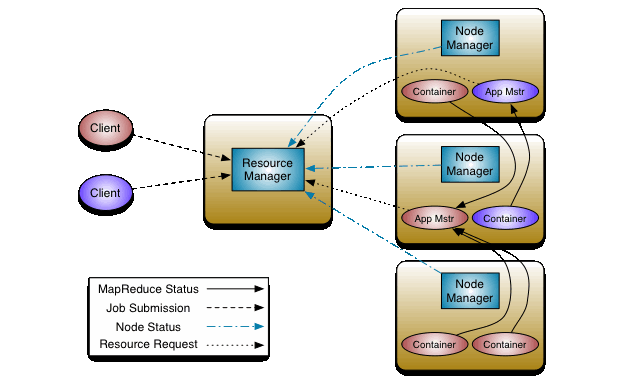
\includegraphics[width=\columnwidth]{./images/yarn_architecture.png}
	\caption[Architektur von YARN]{Architektur von YARN \cite{HadoopYarnArch271}}
	\label{fig:yarnarch}
\end{figure}

Die Kernidee der Architektur von \textbf{YARN} ist die Trennung vom Ressourcenmanagement und Scheduling. Dazu besitzt der Master bzw. \emph{Controller} den \ac{RM}, welcher für das gesamte System zuständig ist und die Anwendungen im System verteilt und überwacht und somit auch als \emph{Load-Balancer} agiert. Er besteht aus zwei Kernkomponenten, dem \ac{AM} und dem \emph{Scheduler}. Der \ac{AM} ist für die Annahme und Ausführung von einzelnen Anwendungen zuständig, denen der Scheduler die dafür notwendigen Ressourcen im Cluster zuteilt.

Jeder Slave-\emph{Node} im Hadoop-Cluster besitzt einen \ac{NM}, welcher für die Überwachung der Ressourcen des Nodes zuständig ist und diese dem \ac{RM} mitteilt. Jede Anwendung besitzt jeweils einen eigenen \ac{AppMstr}, welcher für das anwendungsbezogene Monitoring und die Kommunikation mit dem \ac{RM} und \ac{NM} zuständig ist und die dazu notwendigen Informationen bereit stellt. Jede YARN-Anwendung bzw. Job besteht aus mehreren \emph{Containern}, in denen die einzelnen Tasks der Anwendung auf einem beliebigen Node ausgeführt werden. Auch der \ac{AppMstr} wird dadurch in einem eigenen Container ausgeführt. Das Monitoring der einzelnen Container wird geteilt durchgeführt. Der \ac{NM} übernimmt das Monitoring der genutzten Ressourcen, der jeweilige \ac{AppMstr} die anwendungsbezogenen Monitoring-Aufgaben \cite{HadoopYarnArch271}.

Hadoop enthält zudem einen sog. Timeline-Server. Er ist speziell dafür entwickelt, die Metadaten und Logs der YARN-Anwendungen zu speichern und jederzeit, also auch speziell als Anwendungshistorie, auszugeben \cite{HadoopYarnTlServer271}.

\begin{figure}
    \centering
    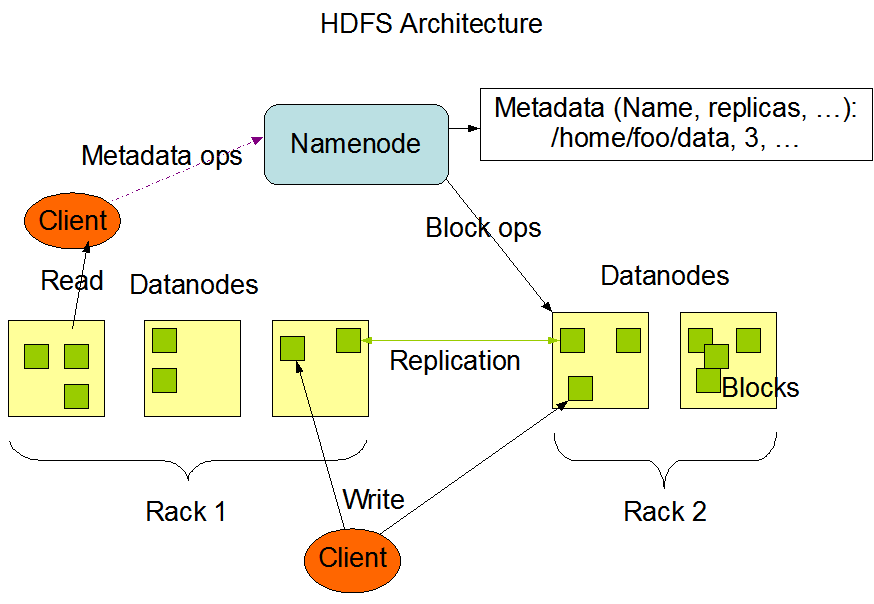
\includegraphics[width=.8\columnwidth]{./images/hdfsarchitecture.png}
    \caption[Architektur des HDFS]{Architektur des HDFS \cite{HadoopHdfsDesc271}}
    \label{fig:hdfsarch}
\end{figure}

Das \textbf{HDFS} basiert auf der gleichen Architektur wie YARN und besitzt ebenfalls einen Master und mehrere Slaves, welches in der Regel die gleichen Nodes sind wie bei YARN sind. Der \emph{NameNode} ist als Master für die Verwaltung des Dateisystems zuständig und reguliert den Zugriff auf die darauf gespeicherten Daten. Die Daten selbst werden in mehrere Blöcke aufgeteilt auf den \emph{DataNodes} gespeichert. Um den Zugriff auf die Daten im Falle eines Node-Ausfalls zu gewährleisten, wird jeder Block auf anderen Nodes repliziert. Dateioperationen (wie Öffnen oder Schließen) werden direkt auf den DataNodes ausgeführt, sie sind darüber hinaus auch dafür verantwortlich, dass Clients die Daten lesen oder beschreiben können \cite{HadoopHdfsDesc271}.

\textbf{MapReduce} bietet analog zu YARN die Möglichkeit, Anwendungen mit einem großen Ressourcenbedarf, welche große Datenmengen verarbeiten, auf einem gesamten Cluster auszuführen. Dazu werden bei einem MapReduce-Job die Eingabedaten aufgeteilt, anschließend von den sog. \emph{Map Tasks} verarbeitet und deren Ausgaben von den sog. \emph{Reduce Tasks} geordnet. Für die Ein- und Ausgabe der Daten wird in der Regel das HDFS, für die Ausführung der einzelnen Tasks YARN genutzt \cite{HadoopMapRedTutorial271}. MapReduce kann man auch als Vorgänger von YARN ansehen, da YARN auch als \emph{MapReduce Next Gen} bzw. \emph{MRv2} bezeichnet wird und aufgrund der API-Kompatibilität von YARN jede MapReduce-Anwendung in der Regel auch auf YARN ausgeführt werden kann \cite{HadoopYarnArch271,HadoopYarnOverview271}.


\section{Adaptive Komponente in Hadoop}\label{sec:inriaSetting}

Eine normale Hadoop-Installation besitzt keine adaptive Komponente, sondern rein statische Einstellungen. Um damit Hadoop zu optimieren, müssen die Einstellungen immer manuell auf den jeweils benötigten Anwendungstyp angepasst werden. Dazu gibt es auch bereits verschiedene Scheduler, den \emph{Fair Scheduler}, welcher alle Anwendungen ausführt und ihnen gleich viele Ressourcen zuteilt, und den \emph{Capacity Scheduler}. Letzterer sorgt dafür, dass nur eine bestimmte Anzahl an Anwendungen pro Benutzter gleichzeitig ausgeführt wird und teilt ihnen so viele Ressourcen zu, wie benötigt werden bzw. der Benutzter nutzen darf. Entwickelt wurde der Capacity Scheduler vor allem für Cluster, die von mehreren Organisationen gemeinsam verwendet werden und sicherstellen soll, dass jede Organisation eine Mindestmenge an Ressourcen zur Verfügung hat \cite{HadoopCapScheduler271}.

Je nach Bedarf besitzt der Capacity Scheduler entsprechende Einstellungen, um \zB den verfügbaren Speicher pro Container festzulegen. Eine weitere Einstellung des Schedulers ist \acl{MARP}, auch \acs{MARP} gennant\acused{MARP}, der angibt, wie viele Prozent der gesamten Ressourcen durch \ac{AppMstr}-Container genutzt werden dürfen \cite{HadoopCapScheduler271}. Damit bewirkt diese Einstellung indirekt auch die maximale Anzahl an Anwendungen, die gleichzeitig ausgeführt werden dürfen. Da der \ac{MARP}-Wert jedoch nicht während der Laufzeit dynamisch angepasst werden kann, haben \citeauthor{zhang2016} in \cite{zhang2016} einen Ansatz zur dynamischen Anpassung des \ac{MARP}-Wertes zur Laufzeit von Hadoop vorgestellt. Dadurch wird der \ac{MARP}-Wert abhängig von den ausgeführten Anwendungen adaptiv zur Laufzeit angepasst, sodass immer möglichst viele Anwendungen gleichzeitig ausgeführt werden können. Dadurch werden Anwendungen im Schnitt um bis zu 40 \% schneller ausgeführt \cite{zhang2016}.

\begin{figure}
    \centering
    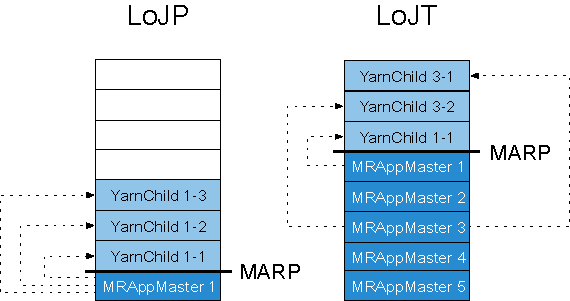
\includegraphics[width=.8\columnwidth]{./images/marpValue.pdf}
    \caption[LoJP und LoJT in Hadoop]{LoJP und LoJT in Hadoop (entnommen aus \cite{zhang2016})}
    \label{fig:marpValue}
\end{figure}

Der Hintergrund dieser \emph{Selfbalancing-Komponente} ist der, dass durch den \ac{MARP}-Wert der für die Anwendungen verfügbare Speicher in zwei Teile aufgeteilt wird. Im einen Teil befinden sich alle derzeit ausgeführten \ac{AppMstr}, im anderen Teil die von den Anwendungen benötigten weiteren Container. Wie groß der Teil für die \ac{AppMstr} ist, wird nun durch den \ac{MARP}-Wert bestimmt. Ist der \ac{MARP}-Wert zu klein, können nur wenige \ac{AppMstr} (und damit Anwendungen) gleichzeitig ausgeführt werden (\emph{Loss of Jobs Parallelism}, LoJP). Ist der \ac{MARP}-Wert jedoch zu groß, können für die ausgeführten Anwendungen nur wenige Container bereitgestellt werden, wodurch sich die Ausführung für eine Anwendung wesentlich verlangsamt (\emph{Loss of Job Throughput}, LoJT)\cite{zhang2016}. \autoref{fig:marpValue} illustriert beide Situationen, wodurch einerseits viel Speicher für weitere Anwendungscontainer ungenutzt bleiben kann, andererseits aber zahlreiche \ac{AppMstr} ohne laufende Anwendungscontainer Speicher unnötig belegen können.

Die Selfbalancing-Komponente passt daher den \ac{MARP}-Wert abhängig von der Speicherauslastung dynamisch zur Laufzeit an. So wird der \ac{MARP}-Wert verringert, wenn die Speicherauslastung sehr hoch ist, und erhöht, wenn die Speicherauslastung sehr niedrig ist \cite{zhang2016}. Dadurch wird es ermöglicht, dass die maximal mögliche Anzahl an Anwendungen ausgeführt werden kann. Die Evaluation von \citeauthor{zhang2016} ergab zudem, dass die dynamische Anpassung des \ac{MARP}-Wertes zudem auch effizienter ist als eine manuelle, statische Optimierung.


\section{Umsetzung des realen Clusters}\label{sec:aufbauCluster}

\citeauthor{zhang2016} haben im Rahmen ihrer gesamten Forschungsarbeit die Open"=Source"=Plattform Hadoop-Benchmark entwickelt und auf Github zur Verfügung gestellt.\footnote{\url{https://github.com/Spirals-Team/hadoop-benchmark}} Sie wurde speziell zum Einsatz in der Forschung erstellt und kann jederzeit an die eigenen Bedürfnisse angepasst werden. Zur Umsetzung des realen Clusters im Rahmen dieser Masterarbeit wurde daher eine speziell angepasste Version der Plattform eingesetzt.

\subsection{Plattform Hadoop-Benchmark}\label{sec:hadoopBenchmark}

Die Plattform ist in mehrere Szenarien unterteilt, darunter ein Hadoop in der Version 2.7.1 ohne Änderungen und ein darauf basierendes Szenario mit der Selfbalancing-Komponente. Hadoop-Benchmark basiert auf der Software \emph{Docker}\footnote{\url{https://www.docker.com/}} und dem dazugehörigen Tool \emph{Docker Machine}, um damit einfach und schnell ein Hadoop-Cluster aufbauen zu können. Mit \emph{Graphite}\footnote{\url{https://graphiteapp.org/}} ist zudem ein Monitoring-Tool enthalten, mit dem die Performance des Clusters überwacht und analysiert werden kann.

\begin{figure}
    \centering
    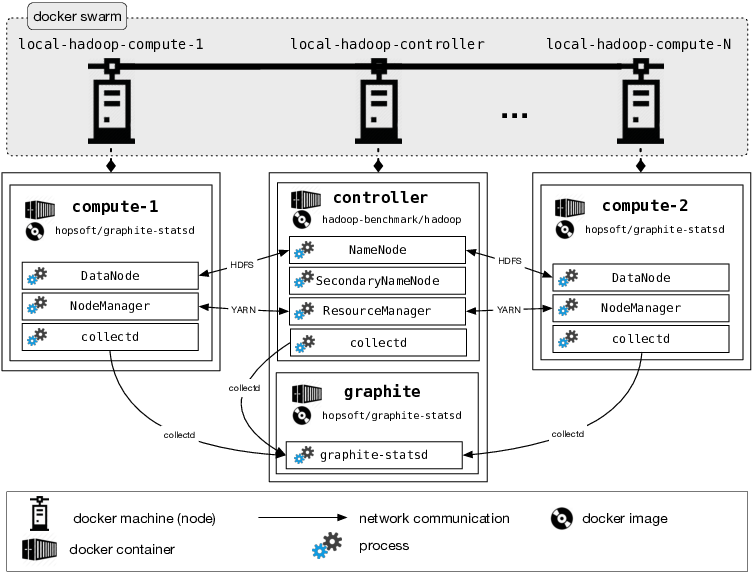
\includegraphics[width=.8\columnwidth]{./images/hadoopBenchmarkArch.png}
    \caption[High-Level-Architektur von Hadoop-Benchmark]{High-Level-Architektur von Hadoop-Benchmark \cite{abb:hadoopBenchmarkArch}}
    \label{fig:hadoopBenchmarkArchitecture}
\end{figure}

\autoref{fig:hadoopBenchmarkArchitecture} zeigt die grundlegende Architektur der Plattform, die mithilfe eines Docker-Swarms auf mehreren \emph{Docker Machines} (für den Einsatz von Docker eingerichtete virtuelle Maschinen) ein Cluster erstellt, auf denen dann in den Docker-Containern das eigentliche Hadoop-Cluster ausgeführt wird. Jeder Hadoop-Container enthält zudem das Tool \emph{collectd}\footnote{\url{https://collectd.org/}}, was das Monitoring des Containers auf Systemebene übernimmt und die Daten an den Graphite-Container auf der Controller-Machine übermittelt. Es ist dabei möglich, eine beliebige Anzahl an Nodes zu nutzen. Auch ist es möglich, den Docker Machines einen beliebig großen Arbeitsspeicher zur Verfügung zu stellen.

Die Plattform Hadoop-Benchmark enthält zudem einige Benchmark-Anwendungen:

\begin{itemize}[noitemsep]
    \item Hadoop Mapreduce Examples
    \item Intel HiBench\footnote{\url{https://github.com/intel-hadoop/HiBench}}
    \item SWIM (Statistical Workload Injector for Mapreduce)\footnote{\url{https://github.com/SWIMProjectUCB/SWIM}}
\end{itemize}

Eine Besonderheit bildet der SWIM-Benchmark, welcher sehr Ressourcenintensiv ist und daher auf einem \emph{Single Node Cluster}, also einem kompletten Hadoop-Cluster auf nur einem Computer, sehr zeitintensiv sein kann. Der Intel HiBench-Benchmark besteht aus Kategorien wie \emph{Machine Learning} oder Graphen, welche wiederum aus einen oder mehreren \emph{Workloads} bestehen, welche entsprechende Anwendungen bzw. Algorithmen auf dem Hadoop-Cluster ausführen. Einige der Hibench-Workloads basieren auf den Mapreduce Examples, welche wiederum voneinander unabhängige Beispielanwendungen für Hadoop darstellen.

\subsection{Anpassungen und Setup}\label{sec:clusterFallstudie}

Da mithilfe der Plattform Hadoop-Benchmark die Erstellung eines Hadoop-Clusters massiv vereinfacht wird, kommt die Plattform auch in dieser Masterarbeit zum Einsatz. Da Docker und Hadoop aber vor allem für den Einsatz in einer Linux-Umgebung entwickelt wurden, wird dazu ein eigener PC mit Ubuntu 16.04 LTS genutzt. Da \sS das .NET-Framework, und damit Windows, benötigt, wird dafür ebenfalls ein eigener PC verwendet. Im konkreten Versuchsaufbau wird für Windows eine VM genutzt, welche auf einem anderen PC als das Cluster ausgeführt wird. Die genauen Spezifikationen der PCs und der Windows-VM sind in \autoref{tab:pcSpecs} aufgelistet. Die Windows-VM und der Cluster-PC werden mithilfe von SSH-Verbindungen miteinander verbunden.

\begin{table}
    \centering
    \begin{tabular}{|c|c|c|c|}
    	\hline
    	 \textbf{}   & \textbf{Cluster-PC} &         \textbf{VM-PC}          & \textbf{Windows-VM}  \\ \hline\hline
    	\textbf{CPU} & \multicolumn{2}{c|}{Intel Core i5-4570 @ 3,2 GHz x 4} &     4 CPU Cores      \\ \hline
    	\textbf{RAM} &              \multicolumn{2}{c|}{16 GB}               &         8 GB         \\ \hline
    	\textbf{SSD} &       512 GB        &             512 GB              &  $\leq$ 100 GB VHD   \\ \hline
    	\textbf{OS}  &  Ubuntu 16.04 LTS   &        Ubuntu 16.04 LTS         & Windows 10 1709 Edu. \\ \hline
    \end{tabular}
    \caption{Spezifikationen der verwendeten PCs und Windows-VM}
    \label{tab:pcSpecs}
\end{table}

Auf dem Cluster-PC nutzt Docker-Machine zur Erstellung, Verwaltung und Ausführung der VMs die Treiber von VirtualBox 5.2\footnote{\url{https://www.virtualbox.org/}}, zum Abrufen der Daten der REST-API über die SSH-Verbindung wird \emph{curl}\footnote{\url{https://curl.haxx.se/}} genutzt. Für das Cluster werden 4 Nodes, der Controller sowie eine Consul-VM zur internen Verwaltung der Netzwerkverbindungen zwischen den VMs und Docker-Containern erstellt. Der Controller erhält 4 GB RAM, jeder der vier Nodes jeweils 2 GB, für den Consul sind 512 MB ausreichend. Für die Windows-VM wird ebenfalls VirtualBox 5.2 eingesetzt.

%TODO: Link zum angepassten Hadoop-Benchmark?
In keinem Szenario der Plattform Hadoop-Benchmark wird standardmäßig der \ac{TLS} von Hadoop gestartet. Daher wurde für diese Fallstudie basierend auf dem Selfbalancing-Szenario ein neues Szenario erstellt, bei dem der \ac{TLS} gestartet wird. Dadurch ist einerseits die Selfbalancing-Komponente von \citeauthor{zhang2016} aktiv und andererseits besteht die Möglichkeit, für das Monitoring zusätzlich den \ac{TLS} zu nutzen.

Um viele standardmäßige Aufgaben und Möglichkeiten zu vereinfachen, wurde zudem ein eigenes Setup-Script erstellt. Es vereinfacht folgende Aufgaben:

\begin{itemize}[noitemsep]
    \item Starten, Beenden und Löschen des kompletten Clusters mit Hadoop
    \item Starten und Beenden des Docker-Containers eines Nodes
    \item Hinzufügen und Entfernen der Netzwerkverbindung des Docker-Containers eines Nodes
    \item Ausführen der verwendeten Benchmarks
    \item Ausführen von eigenen Befehlen auf dem Docker-Container des Controllers
\end{itemize}

Für die Befehle, die das gesamte Cluster betreffen, wird vom Setup-Script meist auf das in Hadoop-Benchmark enthaltene Start-Script zugegriffen. Die Befehle, welche die Docker-Container der Nodes betreffen, sowie das Ausführen von Befehlen im Controller-Container, werden vom Setup-Script direkt ausgeführt. Für das Starten der Benchmarks werden dagegen die in Hadoop-Benchmark enthaltenen Ausführungs-Scripte der Benchmarks gestartet.